\documentclass[9pt,french,xcolor=table]{beamer}

\usepackage[T1]{fontenc}       
\usepackage[utf8]{inputenc}    % pour les accents (mettre latin1 pour windows au lieu de utf8)
\usepackage{babel}    		   % le document est en français
\usepackage{amsmath}           % un package mathématique
\usepackage{xcolor}            % pour définir plus de couleurs 
    \definecolor{bleu}{HTML}{002060}
    \definecolor{rouge}{HTML}{990000}
\usepackage{graphicx}          % pour insérer des figures
\usepackage{tikz,pgf}
\usepackage{multicol}
\usepackage{caption}
\usepackage{listings,lstautogobble}
\usepackage{multirow}


\usecolortheme[named=bleu]{structure}
\useinnertheme[shadow]{rounded}

\setbeamersize{text margin left=0.6cm}
\setbeamersize{text margin right=0.4cm}
\setbeamersize{text margin left=.5cm, text margin right=.5cm}

\setbeamertemplate{itemize item}[ball]
\setbeamertemplate{itemize subitem}[triangle]
\setbeamertemplate{itemize subsubitem}[circle]

\setbeamertemplate{blocks}[rounded][shadow=true]

\setbeamercolor{title}{fg=white}
\setbeamercolor{author}{fg=white}
\setbeamercolor{institute}{fg=white}
\setbeamercolor{date}{fg=white}
\setbeamercolor{frametitle}{fg=white}
\setbeamercolor{structure}{fg=bleu}
\setbeamercolor{section in toc}{fg=bleu}
\setbeamercolor{block title}{fg=black,bg=blue1}        % titre block normal 
\setbeamercolor{block body}{fg=black,bg=bleu1!50}      % corps block normal
\setbeamercolor{block body alerted}{fg=white,bg=red}   % idem pour un block alerte

% Symboles de navigation des slides
\setbeamertemplate{navigation symbols}{
%       \insertslidenavigationsymbol
%       \insertframenavigationsymbol
%       \insertsubsectionnavigationsymbol
%       \insertsectionnavigationsymbol
%       \insertdocnavigationsymbol
%       \insertbackfindforwardnavigationsymbol
}

\setbeamertemplate{frametitle}{%
    \usebeamerfont{frametitle}\insertframetitle\strut%
    \vskip0.5\baselineskip%
    \vskip0pt%
    \nointerlineskip
}

\title[Titre court]{\Huge \bf Soutenance de TN30}
\author[Jean C4stex]{Jean C4stex}
\institute{Organisme d'acceuil}
\date{\today}

% Meta-donnée du pdf généré
\hypersetup{
%       pdfpagemode = FullScreen,% afficher le pdf en plein écran
      pdfauthor   = {Moi}%
      pdftitle    = {Soutenance stage ST30},%
      pdfsubject  = {Mon super sujet},%
      pdfkeywords = {Soutenance,Informatique,LaTeX},%
      pdfcreator  = {PDFLaTeX},%
      pdfproducer = {PDFLaTeX}%
}

% Sommaire
\AtBeginSection[]{
    \begin{frame}
        \frametitle{\vspace*{0.45cm} \huge \bf Sommaire }
        \begin{center}
            \centering
            \tableofcontents[currentsection,hideothersubsections]
        \end{center}
    \end{frame}
}

\AtBeginSubsection[]{
    \begin{frame}
        \frametitle{\vspace*{0.45cm} \huge \bf Sommaire }
        \begin{center}
            \centering
            \tableofcontents[currentsection,currentsubsection]
        \end{center}
    \end{frame}
}

\begin{document}
	% page de titre
	\begin{frame}
	  \pgfputat{\pgfxy(-0.5,0.9)}{\pgfbox[left,top]{\pgfimage[width=\paperwidth,height=\paperheight ]{./assets/title1.pdf}}}
      \vspace*{1.6cm}
      \begin{center}
        \titlepage
      \end{center}
	\end{frame}

	% Setup du fond et du pied de page
	\setbeamertemplate{background canvas}{
        
\includegraphics[width=\paperwidth,height=\paperheight]{./assets/slide.pdf}
	}
	\addtobeamertemplate{footline}{
		\vspace{-0.35cm}
		\begin{flushleft}
			\hspace{0.1cm}
			{\color{white} \insertframenumber/\inserttotalframenumber\hfill\insertsection}
			\hspace{-0.1cm}
		\end{flushleft}
	}
	
	% Sommaire
	\begin{frame}%[allowframebreaks] % Dé-commenter s'il y a beaucoup de section
		\frametitle{\vspace*{0.45cm} \huge \bf Sommaire }
        \begin{center}
            \centering
            \tableofcontents[]
        \end{center}
	\end{frame}

\section{Introduction}
    \begin{frame}[c]
        \frametitle{\vspace*{0.45cm} \huge \bf Introduction}
        \vspace*{0.45cm}
        \begin{itemize}
            \item Mise en contexte du sujet
            \item Blabla introductif
        \end{itemize}
        \begin{multicols}{2}
            \begin{figure}
                \centering
                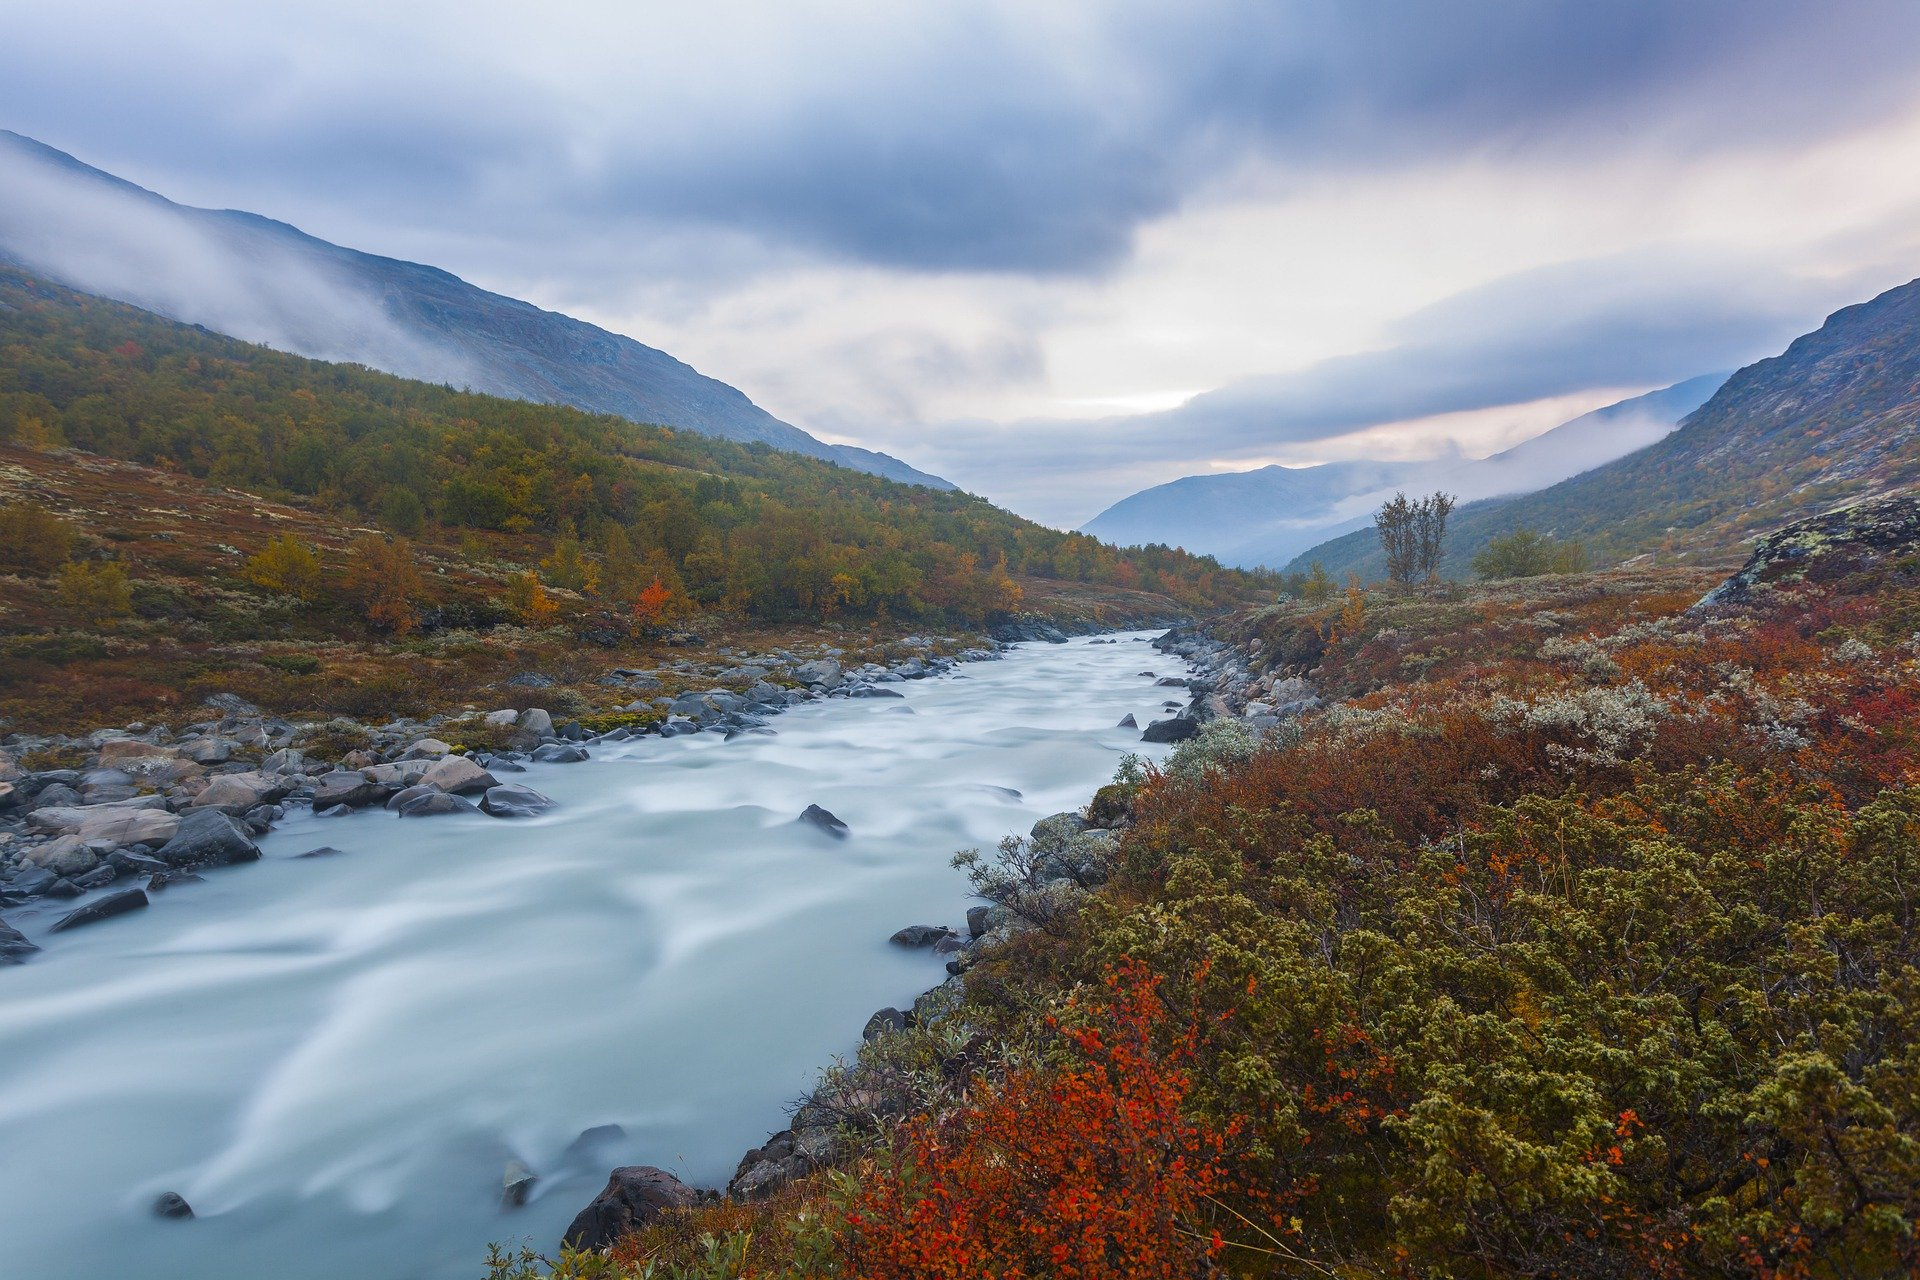
\includegraphics[width=0.8\linewidth]{./img/image.jpg}
                \caption{Une belle photo montrant l'endroit où je n'ai pas passé mon stage.}
            \end{figure}
            \columnbreak
            \begin{itemize}
                \item Blabla introductif:
                \begin{itemize}
                    \item Item 1
                    \item Item 2
                \end{itemize}
            \end{itemize}
        \end{multicols}
    \end{frame}
    
\section{Revue de la littérature}
    \begin{frame}[c]
        \frametitle{\vspace*{0.45cm} \huge \bf Revue de la littérature}
        \begin{itemize}
            \item Mise en problématique du sujet de stage
            \item Blabla résumant les travaux antécédants et la revue scientifique et/ou opérationnelle
        \end{itemize}
    \end{frame}
    
\section{Contribution}
    \begin{frame}[c]
        \frametitle{\vspace*{0.45cm} \huge \bf Contribution}
        \begin{itemize}
            \item Blabla résumant les travaux effectuées 
            \item Blabla sur la méthodologie choisie
            \item Blabla sur les problèmes rencontrés et les solutions /pistes de solutions apportées
            \item Blabla sur l'évaluation de ses travaux et discussion des résultats
        \end{itemize}
    \end{frame}
        
\section{Conclusion}
    \begin{frame}[c]
        \frametitle{\vspace*{0.45cm} \huge \bf Conclusion}
        \vspace*{0.5cm}
        \begin{itemize}
            \item Blabla sur pourquoi ce stage était très enrichissant sur le plan personnel et méthodologique
            \item Blabla critique sur ses résultats, points d'améliorations
            \item Blabla sur la mise en relation des résultats obtenus avec la problématique définie
            \item Ouverture
        \end{itemize}
    \end{frame}
    
\section{Bibliographie}
    \begin{frame}[allowframebreaks]
        \frametitle{\vspace*{0.45cm} \huge \bf Références}
        \vspace*{0.5cm}
        \nocite{*}
        \bibliographystyle{amsalpha}
        \bibliography{./references.bib}
    \end{frame}    
\end{document}
